\documentclass[11pt]{article}
\usepackage[margin=2.2cm]{geometry}
\usepackage{amsmath,amssymb,booktabs,tikz}
\usetikzlibrary{arrows.meta}
\title{Precision of the $V\to q\bar q g$ evaluator on the LHC $Z$+jet phase space}
\date{}
\begin{document}
\maketitle

\paragraph{Variables.} In a production region $A>1$ ($A=x,y,z$; the other two invariants are negative) we use
\[
  v=\frac1A=\frac{q^2}{\hat s},\qquad u=-\frac bA,\qquad w=-\frac cA=1-u-v,\qquad u,v,w>0,
\]
for region $z$: $u=-y/z$, $w=-x/z$ (the package's region triangle is $(X,Y)=(w,u)$, $Z=v$). With $E_j,\theta$ the jet
energy and angle in the partonic frame, $u=E_j(1+\cos\theta)/\sqrt{\hat s}$ and $w=E_j(1-\cos\theta)/\sqrt{\hat s}$, so
\[
  \frac{p_T^2}{M_Z^2}=\frac{u\,w}{v},\qquad \frac uw=e^{2\eta^*},\qquad \sqrt{\hat s}=\frac{M_Z}{\sqrt v}\qquad(q^2=M_Z^2),
\]
with $\eta^*$ the jet rapidity in the partonic frame. Every edge of the triangle is a physical limit:
\begin{itemize}
\item \textbf{Threshold}, $v\to1$: then $u+w\to0$, so $p_T\to0$.
\item \textbf{Collinear}, $u\to0$ or $w\to0$: $p_T\to0$, or a forward jet ($|\eta^*|\to\infty$).
\item \textbf{High energy}, $v\to0$.
\end{itemize}

\paragraph{The LHC domain.} We take
$15\,\text{GeV}<p_T<2\,\text{TeV}$, $\sqrt{\hat s}\le13.6$ TeV (the collider energy) and the jet acceptance
$|\eta^*|\le4.5$. In $(u,v)$, with $\kappa_1=(15/91.19)^2=0.0271$ and $\kappa_2=(2000/91.19)^2=481$:
\[
  \kappa_1\,v\;\le\;u\,w\;\le\;\kappa_2\,v,\qquad v\ge\Big(\frac{M_Z}{13.6\,\text{TeV}}\Big)^2=4.5\cdot10^{-5},\qquad
  e^{-9}\le\frac uw\le e^{9}.
\]
The $p_T$ cut keeps away from threshold, $v\le1+2\kappa_1-2\sqrt{\kappa_1+\kappa_1^2}=0.72$. The rapidity cut keeps away
from the collinear edges, $u,w\ge1.2\cdot10^{-4}$. Without it, the $p_T$ cut alone allows $u,w$ down to
$\kappa_1v_{\min}\approx1.2\cdot10^{-6}$: a 15 GeV jet at the highest energies, with $\eta^*\approx7$.
The rapidity cut is applied in the partonic frame. In the high-energy corner, where it matters, the boost of the partonic
system is small ($\le\ln(\sqrt s/\sqrt{\hat s})$), so $\eta^*$ is close to the lab rapidity.

\begin{center}
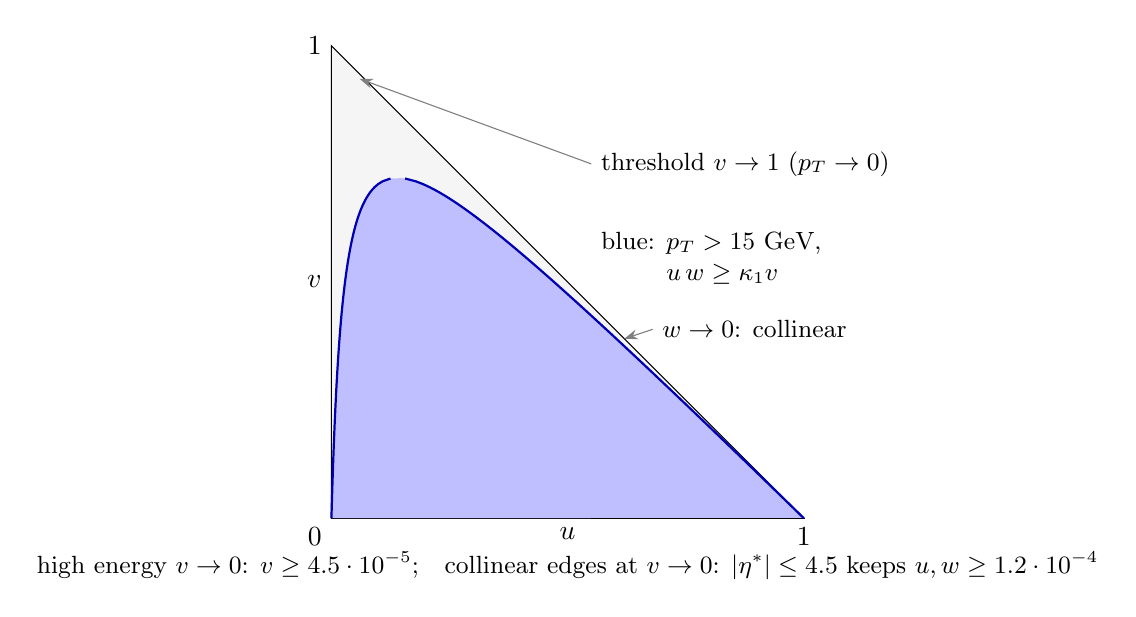
\begin{tikzpicture}[scale=6,>=Stealth]
  \fill[gray!8] (0,0)--(1,0)--(0,1)--cycle; \draw (0,0)--(1,0)--(0,1)--cycle;
  \fill[blue!25,domain=0.00005:0.72,samples=120,variable=\v]
     plot ({((1-\v)-sqrt(max((1-\v)^2-4*0.0271*\v,0)))/2},\v) --
     plot[domain=0.72:0.00005] ({((1-\v)+sqrt(max((1-\v)^2-4*0.0271*\v,0)))/2},\v) -- cycle;
  \draw[blue!70!black,thick,domain=0.00005:0.72,samples=120,variable=\v]
     plot ({((1-\v)-sqrt(max((1-\v)^2-4*0.0271*\v,0)))/2},\v);
  \draw[blue!70!black,thick,domain=0.00005:0.72,samples=120,variable=\v]
     plot ({((1-\v)+sqrt(max((1-\v)^2-4*0.0271*\v,0)))/2},\v);
  \node[below] at (0.5,0) {$u$}; \node[left] at (0,0.5) {$v$};
  \node[below left] at (0,0) {$0$}; \node[below] at (1,0) {$1$}; \node[left] at (0,1) {$1$};
  \node[font=\small,align=left,anchor=west] at (0.55,0.75) {threshold $v\to1$ ($p_T\to0$)};
  \draw[->,gray] (0.55,0.75) -- (0.06,0.93);
  \node[font=\small,align=left,anchor=west] at (0.55,0.55) {blue: $p_T>15$ GeV,\\ \phantom{blue: }$u\,w\ge\kappa_1 v$};
  \node[font=\small,align=left,anchor=west] at (0.68,0.40) {$w\to0$: collinear};
  \draw[->,gray] (0.68,0.40) -- (0.62,0.38);
  \node[font=\small,align=left] at (0.5,-0.1) {high energy $v\to0$: $v\ge4.5\cdot10^{-5}$;\quad
     collinear edges at $v\to0$: $|\eta^*|\le4.5$ keeps $u,w\ge1.2\cdot10^{-4}$};
\end{tikzpicture}
\end{center}
\noindent The energy and rapidity cuts act at the $10^{-4}$ scale, too close to the corners to be seen on this linear
scale.

\begin{center}
\newcommand{\ptpanel}[4]{% kappa, vmax, pTmin, colour
\begin{tikzpicture}[scale=3.9]
  \fill[gray!8] (0,0)--(1,0)--(0,1)--cycle; \draw (0,0)--(1,0)--(0,1)--cycle;
  \fill[#4!30,domain=0.00005:#2,samples=150,variable=\v]
     plot ({((1-\v)-sqrt(max((1-\v)^2-4*#1*\v,0)))/2},\v) --
     plot[domain=#2:0.00005] ({((1-\v)+sqrt(max((1-\v)^2-4*#1*\v,0)))/2},\v) -- cycle;
  \draw[#4!70!black,thick,domain=0.00005:#2,samples=150,variable=\v]
     plot ({((1-\v)-sqrt(max((1-\v)^2-4*#1*\v,0)))/2},\v);
  \draw[#4!70!black,thick,domain=0.00005:#2,samples=150,variable=\v]
     plot ({((1-\v)+sqrt(max((1-\v)^2-4*#1*\v,0)))/2},\v);
  \draw[dashed,gray] (0,#2) -- (1-#2,#2);
  \node[left,font=\scriptsize] at (0,#2) {$#2$};
  \node[below,font=\small] at (0.5,0) {$u$}; \node[left,font=\small] at (0,0.22) {$v$};
  \node[below left,font=\scriptsize] at (0,0) {$0$}; \node[below,font=\scriptsize] at (1,0) {$1$};
  \node[left,font=\scriptsize] at (0,1) {$1$};
  \node[font=\small,align=left,anchor=west] at (0.38,0.86) {$p_T>#3$ GeV\\ $\kappa_1=#1$};
\end{tikzpicture}}%
\ptpanel{0.0271}{0.72}{15}{blue}\hspace{4mm}%
\ptpanel{0.0752}{0.58}{25}{teal}\hspace{4mm}%
\ptpanel{0.1473}{0.47}{35}{orange}
\end{center}
\noindent The domain $u\,w\ge\kappa_1v$ for $p_{T,\min}=15$, 25 and 35 GeV, with $\kappa_1=(p_{T,\min}/M_Z)^2$. The
largest $v$ (dashed), i.e.\ the closest approach to threshold, is 0.72, 0.58 and 0.47. At high energy every cut still
reaches the collinear edges, as $u,w\approx\kappa_1v$; there the rapidity acceptance takes over.

\paragraph{How the accuracy is estimated.} Two different quantities enter.

\emph{1. The error estimate of the double evaluator} (returned by the package with every value):
\[
  \varepsilon_{\rm est}=10\,|R_1-R_2|+\epsilon\sum|\text{terms}|,\qquad \epsilon=10^{-13}.
\]
\begin{itemize}
\item $R_1,R_2$ are two double evaluations of the same point, from the same 27-digit start values, along two different
  complex-deformed integration paths. Their difference catches the path-dependent integration error.
\item $\sum|\text{terms}|$ is the sum of the absolute values of all terms (rational function $\times$ generator $\times$
  multiplier) in the remainder. The second term covers the systematic error of the double system, which is the same
  on every path (its matrices come from a floating-point orthonormalisation), amplified by the cancellation in the
  sum. $\epsilon$ is provisional: the smallest value covering every value checked so far.
\end{itemize}
In all tests this was an upper bound, but about 1000 times too large. Here it only selects the points to check.

\emph{2. The actual error} is the difference from a quad evaluation at the same point:
$|R_{\rm double}-R_{\rm quad}|/|R_{\rm quad}|$. Quad integrates the exact integer system in double-double from the
27-digit start values, and builds the generators, the rational functions and the sums in double-double. It is trusted
to far beyond the $10^{-6}$ level:
\begin{itemize}
\item its own two-path error is $\sim10^{-23}$;
\item it agrees with the exact published planar values to $3\cdot10^{-16}$, the precision of that reference;
\item in the production regions it agrees with a direct integration from the decay to $10^{-23}$.
\end{itemize}

\emph{3. The check} (\texttt{accuracy\_study/pheno\_domain\_check.py}):
\begin{itemize}
\item \textbf{Points:} about 330 per region, log-spaced in $v$ and dense towards both collinear edges.
\item \textbf{Double:} every point, with its estimate. All 84 values are included: 6 helicity coefficients
  ($\alpha_{1,2,3}$, $\gamma_{1,2,3}$) times 14 colour layers.
\item \textbf{Quad:} where the estimate exceeds $10^{-6}$, the three worst points (by estimate) of each band of
  $\min(u,w)$ in each region. That is 9 points per region with the rapidity cut and 15 without.
\item \textbf{Colour sum:} for the colour-summed coefficients ($N_c=3$, $N_f=5$, $N_{f,Z}=1$, the worst of the six)
  we quote the bound $\sum_l|c_l|\,|\delta_l|/|\sum_l c_l\,a_l|$. Here $c_l=N_c^aN_f^bN_{f,Z}^c$ and $\delta_l$ is
  the actual error of layer $l$; by the triangle inequality this is an upper bound.
\end{itemize}

\emph{Limits.}
\begin{itemize}
\item Quad was run only at a selection of points, the worst by estimate. The estimate ranks the points well, but the
  real worst point could be one not checked.
\item $N_{f,Z}=1$ is an arbitrary choice for the colour sum.
\item The colour-sum figure is a bound and can overstate the error.
\item To make the statement airtight, run quad at every point whose estimate exceeds $10^{-6}$: 250--300 points per
  region, 1--2 hours in total.
\end{itemize}

\paragraph{Results.} Error of the colour-summed coefficients in double at the checked points (the worst of each band,
in all three regions):
\begin{center}
\begin{tabular}{lll}
\toprule
$\min(u,w)$ & without rapidity cut & with $|\eta^*|\le4.5$ \\
\midrule
$\ge10^{-3}$ & $10^{-8}$ -- $6\cdot10^{-6}$ & median $1.2\cdot10^{-6}$, worst $3.4\cdot10^{-6}$ \\
$10^{-4}$ -- $10^{-3}$ & $4\cdot10^{-7}$ -- $9\cdot10^{-6}$ & median $1.1\cdot10^{-6}$, worst $8.7\cdot10^{-6}$ \\
$2\cdot10^{-5}$ -- $10^{-4}$ & $3\cdot10^{-5}$ -- $10^{-4}$ & outside the domain \\
$<2\cdot10^{-5}$ & $10^{-3}$ -- $O(1)$ & outside the domain \\
\bottomrule
\end{tabular}
\end{center}
\begin{itemize}
\item \textbf{The failing corner.} At high energy $\min(u,w)\approx p_T^2/\hat s$, so the points that fail ($\min(u,w)
  \lesssim10^{-4}$) are jets with $\sqrt{\hat s}\gtrsim100\,p_T$, i.e.\ $\eta^*\gtrsim4.6$. They are outside the detector
  acceptance, and the rapidity cut removes them.
\item \textbf{Individual colour layers.} Some single layers show relative errors up to $10^{-3}$ even at high $p_T$. They
  are $10^4$--$10^6$ times smaller than the other layers at the same point: relative to the largest value there, the
  error is at most $4\cdot10^{-6}$ (typically $10^{-7}$), and they do not affect the colour sum.
\item \textbf{Where double loses digits.} The sum over rational functions times generators cancels: the sum of
  $|$terms$|$ exceeds the value by $10^4$ in the bulk and up to $10^9$ near the edges. Where double is not enough, quad
  (\texttt{precision='quad'}, 5--10 s per point) keeps 15 or more digits. Near the edges, the corner series is the
  proper tool.
\end{itemize}

\paragraph{Conclusion.} On the LHC domain ($15\,\text{GeV}<p_T<2$ TeV, $\sqrt{\hat s}\le13.6$ TeV, $|\eta^*|\le4.5$) the
double evaluator gives the colour-summed coefficients to better than $10^{-5}$ in all three regions: typically
$10^{-6}$, at worst $9\cdot10^{-6}$, at the forward edge of the acceptance ($p_T=15$--$55$ GeV, $\min(u,w)\approx10^{-4}$)
and at the highest $p_T$ and energy ($p_T\approx1.4$ TeV, $\sqrt{\hat s}=13.6$ TeV). Relative to the largest of the 84
values at a point, the error is at most $4\cdot10^{-6}$. A strict $10^{-6}$ everywhere needs quad at those points.

\end{document}
